% !TEX root = poster.tex
\headerbox{\textbf{Flavour Tagging in Run I}}{name=run1,column=1,span=2,row=0}{
\begin{minipage}{0.474\boxwidth}
\textbf{Strategy}\\[-0.35em]
\begin{itemize}
\setlength\itemsep{0.01em}
\vspace{-0.3em}
\item for each tagger one calibration valid for all channels 
\item systematic uncertainties from
\begin{itemize}
\setlength\itemsep{0.01em}
\setlength{\itemindent}{-.11in}
\vspace{-0.4em}
\item[${\color{tu_gruen}-}$] calibration methods
\item[${\color{tu_gruen}-}$] results in different control channels 
\end{itemize}
\vspace{-0.4em}
\item "ad-hoc" calibration from specific control channels for analyses dominated by FT uncertainty %(\BdToJPsiKS)
\end{itemize}
\vspace{-0.9em}
%\begin{center}
%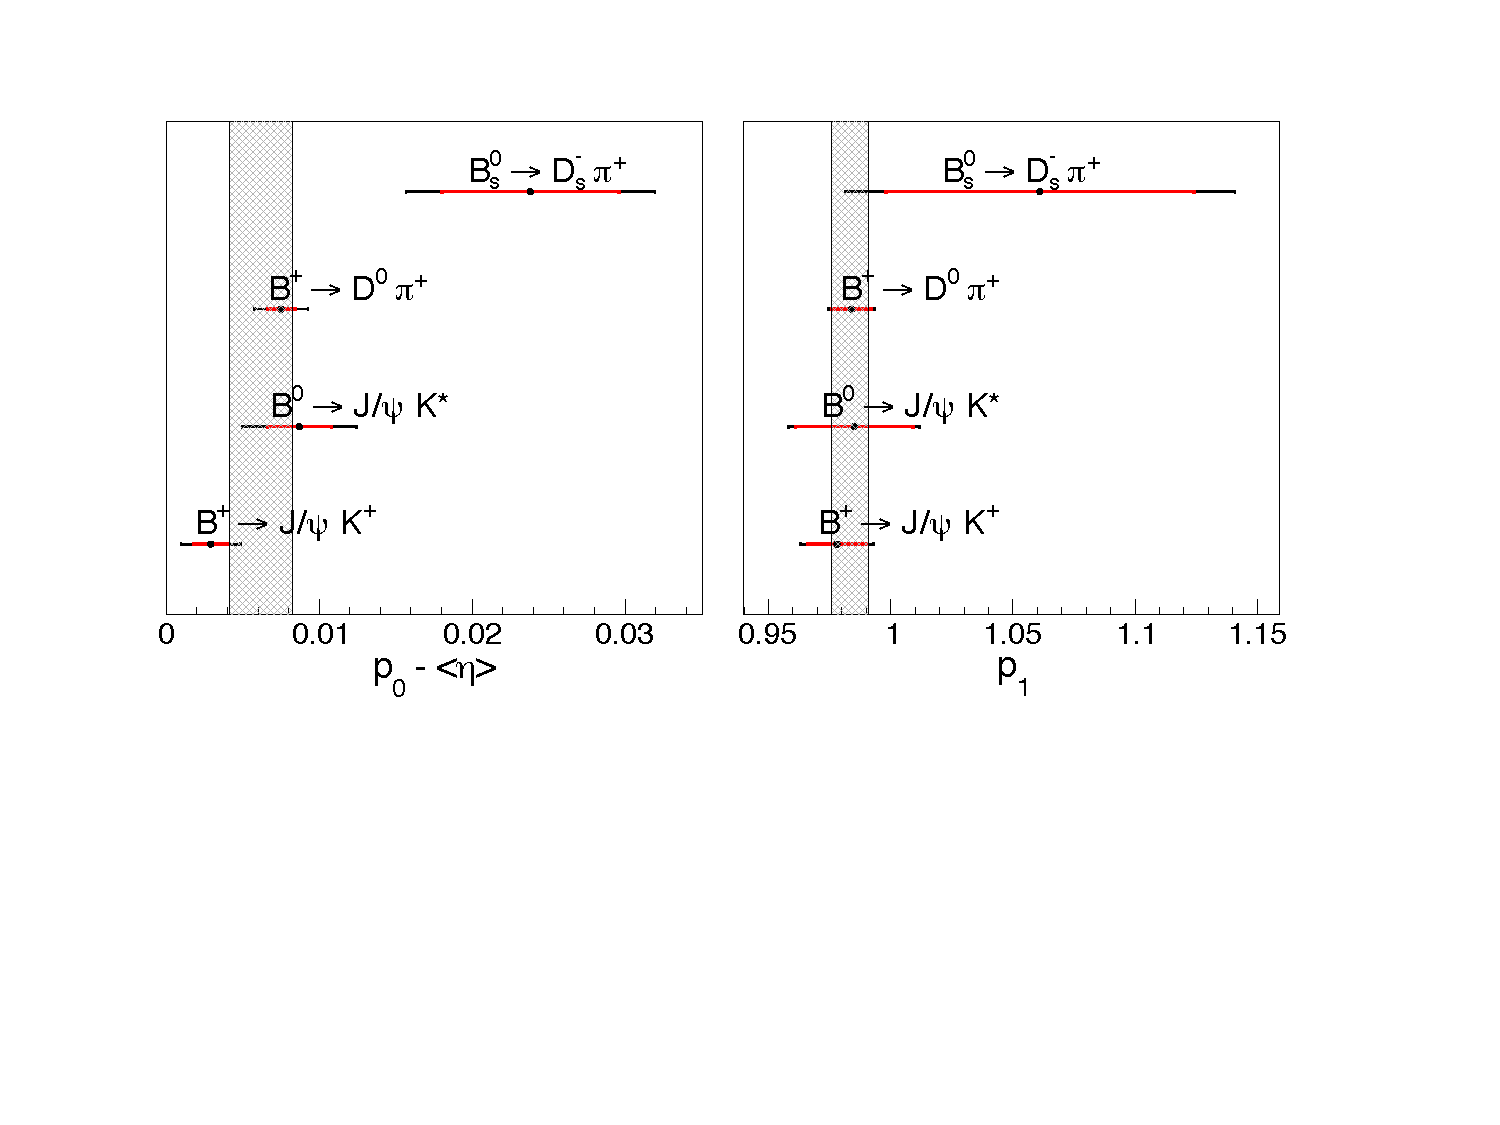
\includegraphics[width=0.466\boxwidth]{graphP0P1.pdf}
%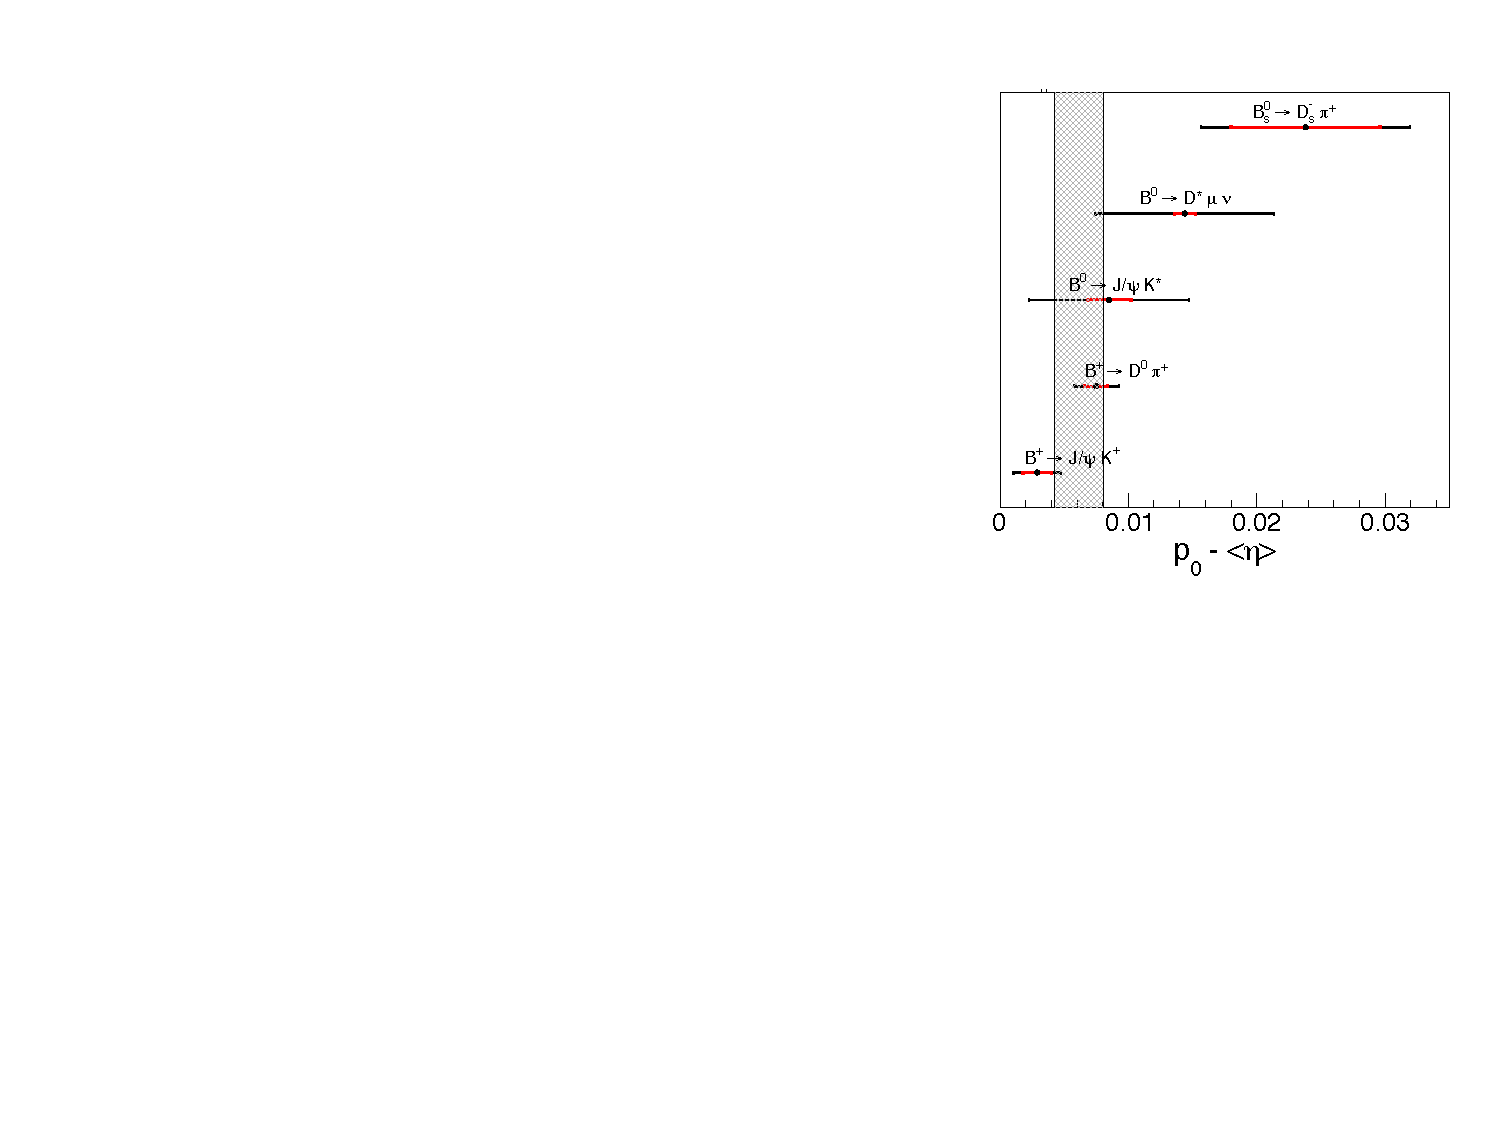
\includegraphics[width=0.233\boxwidth]{portability_p0.pdf}
%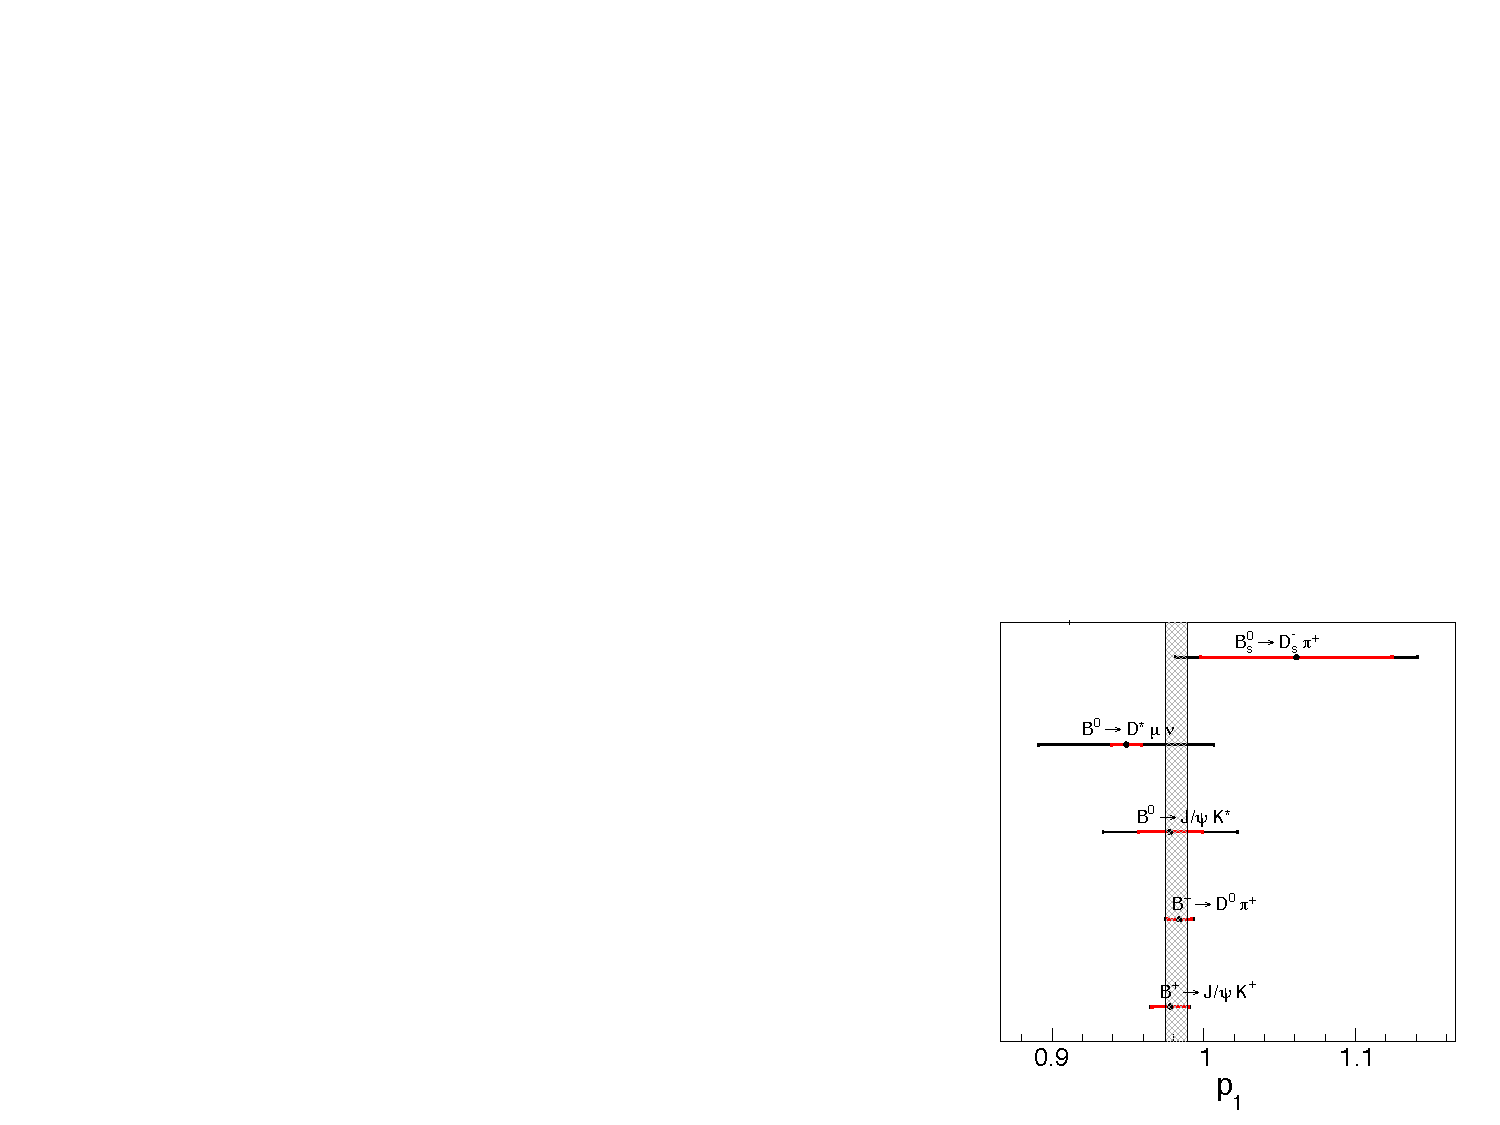
\includegraphics[width=0.233\boxwidth]{portability_p1.pdf}
%\end{center}
\vspace{1.15em}
\textbf{Performance in analyses}
\begin{center}
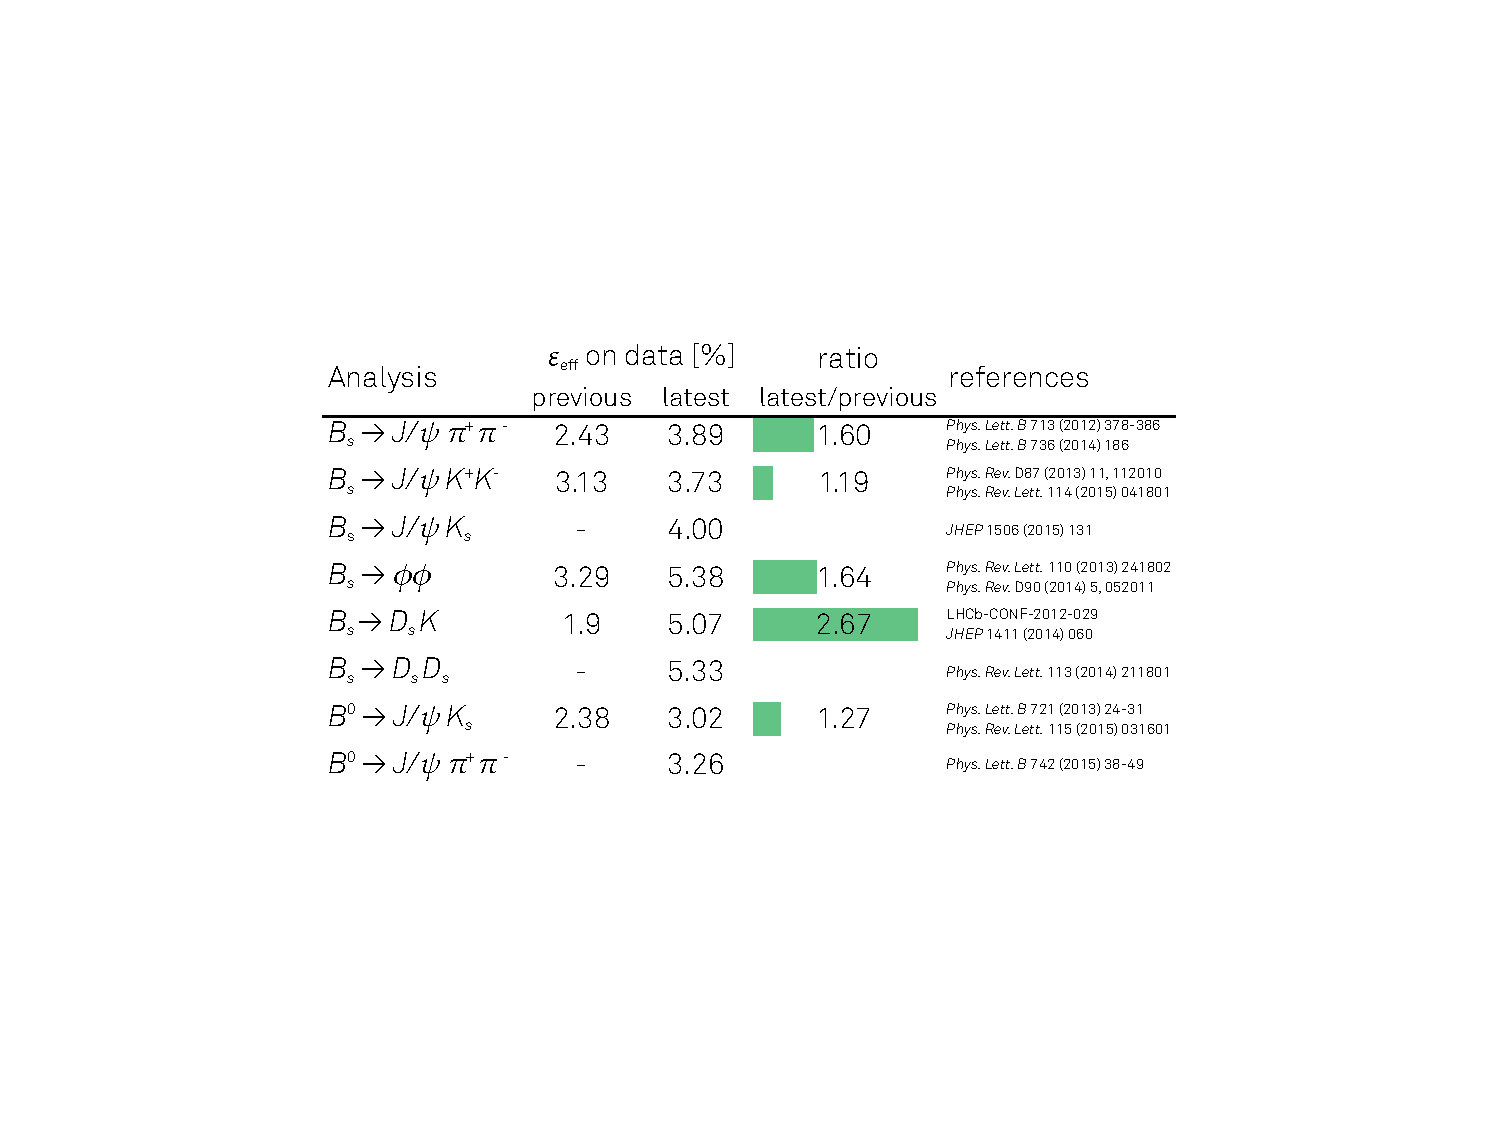
\includegraphics[width=1.00\textwidth]{figures/table_improvement.pdf}
\end{center}
\textbf{Performance improvements in Run I}
\begin{itemize}
\setlength\itemsep{0.01em}
\vspace{-0.3em}
\item OS tagging improved $\mathcal{O}$(15\%) 
\item SS kaon tagging improved $\mathcal{O}$(40\%)
\vspace{0.5em}
\setlength{\itemindent}{.14in}
\item[$\color{tu_gruen}\Rightarrow$] \textbf{Flavour Tagging has been a success in Run I}
\end{itemize}
\end{minipage}
\vspace{0.6em}
\hfill
\begin{minipage}{0.474\boxwidth}
%\vspace{-0.1em}
\textbf{Highlight analyses using flavour tagging}\\
\vspace{-0.05em}\\
%\textbf{Measurement of $\Delta m_s$}\\%[0.5em]
\parbox{0.190\boxwidth}{\textbf{\vspace{0.4em}Measurement of \dms}\\Determination of the\\ $\Bs-\Bsb$ oscillation\\ frequency with\\ \BsToDspi [3].\vspace{0.5em}\\$e^{-\Gamma t}\left(...+\!d\cos\left(\Delta mt\right)\right)$}
\hspace{0.25em}
\parbox{0.474\textwidth}{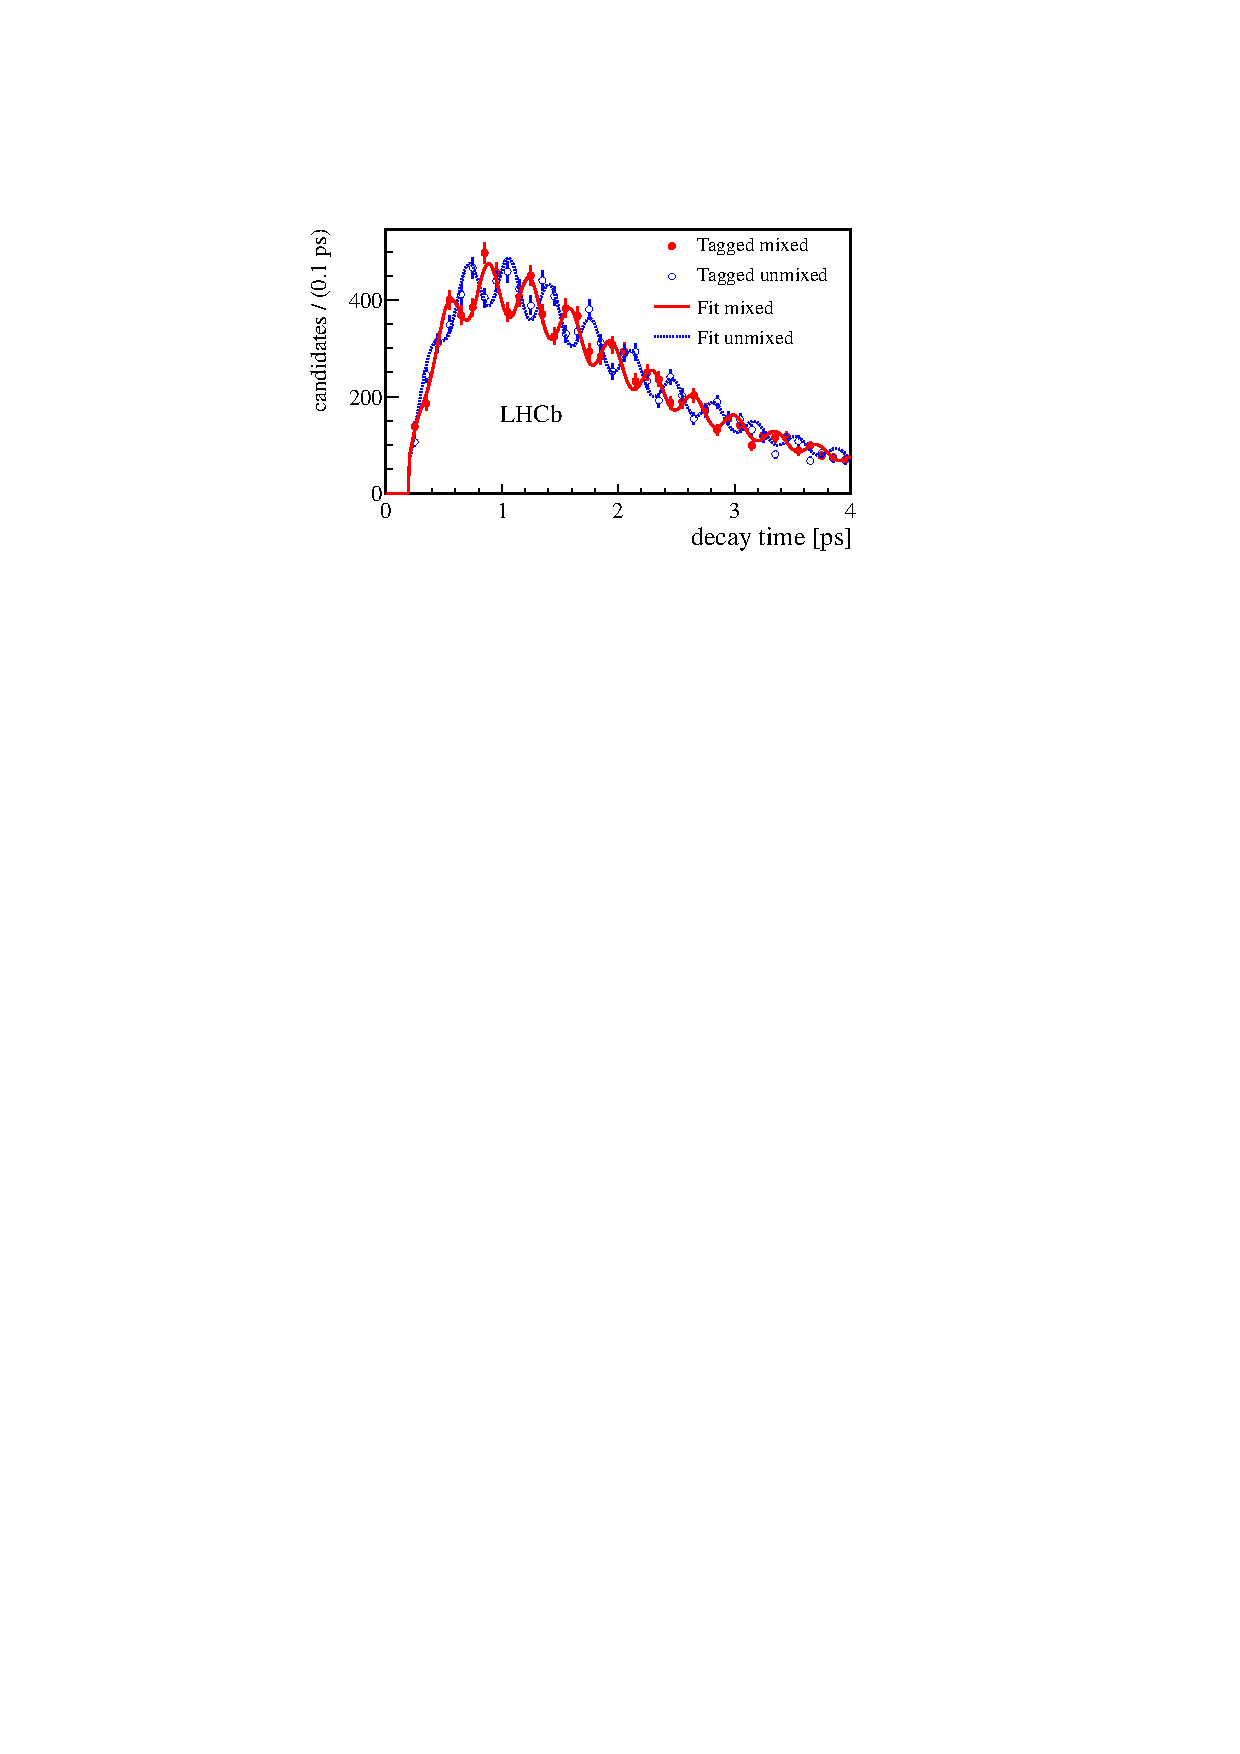
\includegraphics[width=0.266\boxwidth]{Bs_mixing1.pdf}}\\
\vspace{0.25em}\\
\textbf{Measurement of CP ciolation in \BsToDsK decays}\\
\vspace{-0.35em}\\
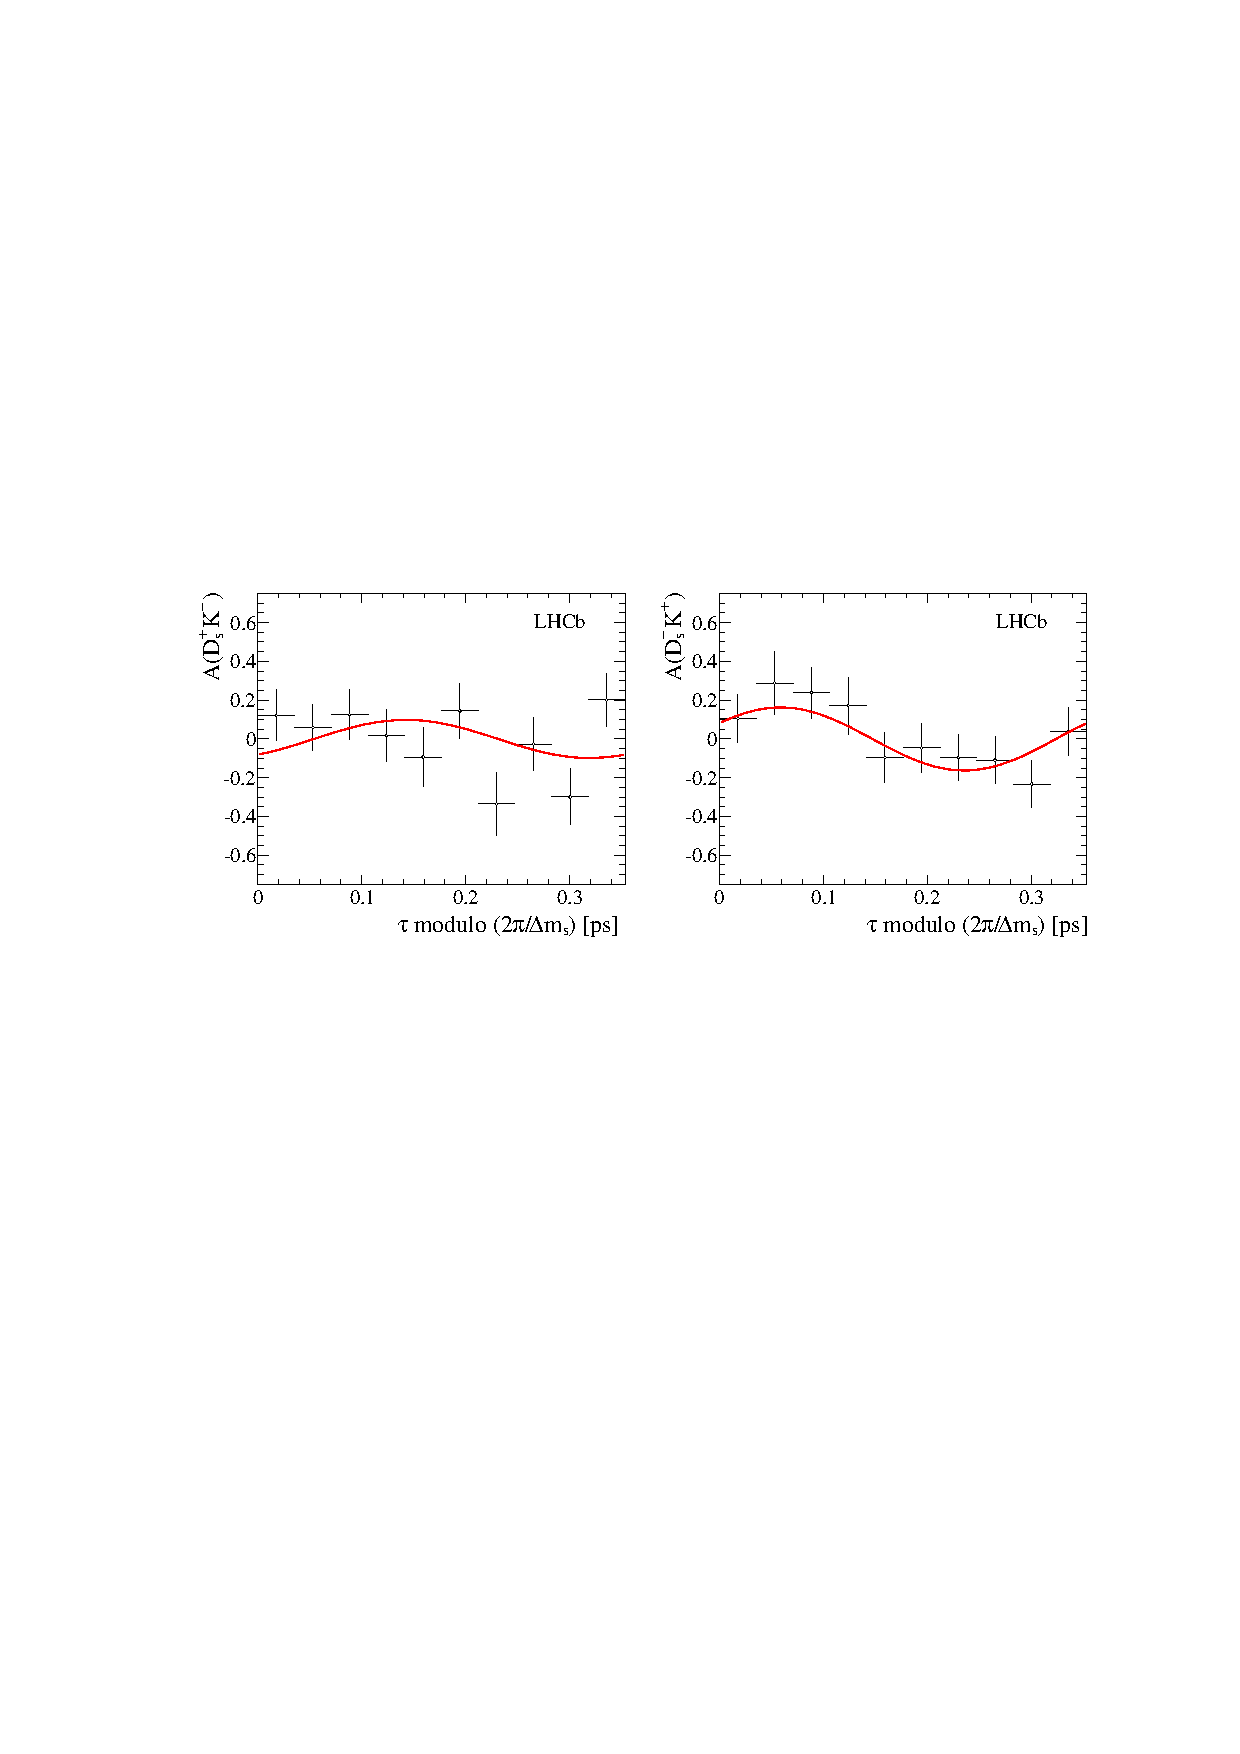
\includegraphics[width=0.98\textwidth]{CPV_DsK.pdf}\\
${\color{tu_gruen}\rightarrow}$ SS kaon nnet adds more than 1.3\, \% to $\varepsilon_\text{eff}$ [4]\\
\vspace{-0.35em}\\
\parbox[c]{0.197\boxwidth}{\textbf{\vspace{0.4em}Measurement of $\sin2\beta$}\\${\color{tu_gruen}\rightarrow}$ precision analysis\\${\color{tu_gruen}\rightarrow}$ "ad-hoc" calibration\\ ${\color{white}\rightarrow}$with \BuToJPsiKp\\${\color{white}\rightarrow}$and \BdToJPsiKst\\${\color{white}\rightarrow}$[5]}
\hspace{0.25em}
\parbox[c]{0.474\textwidth}{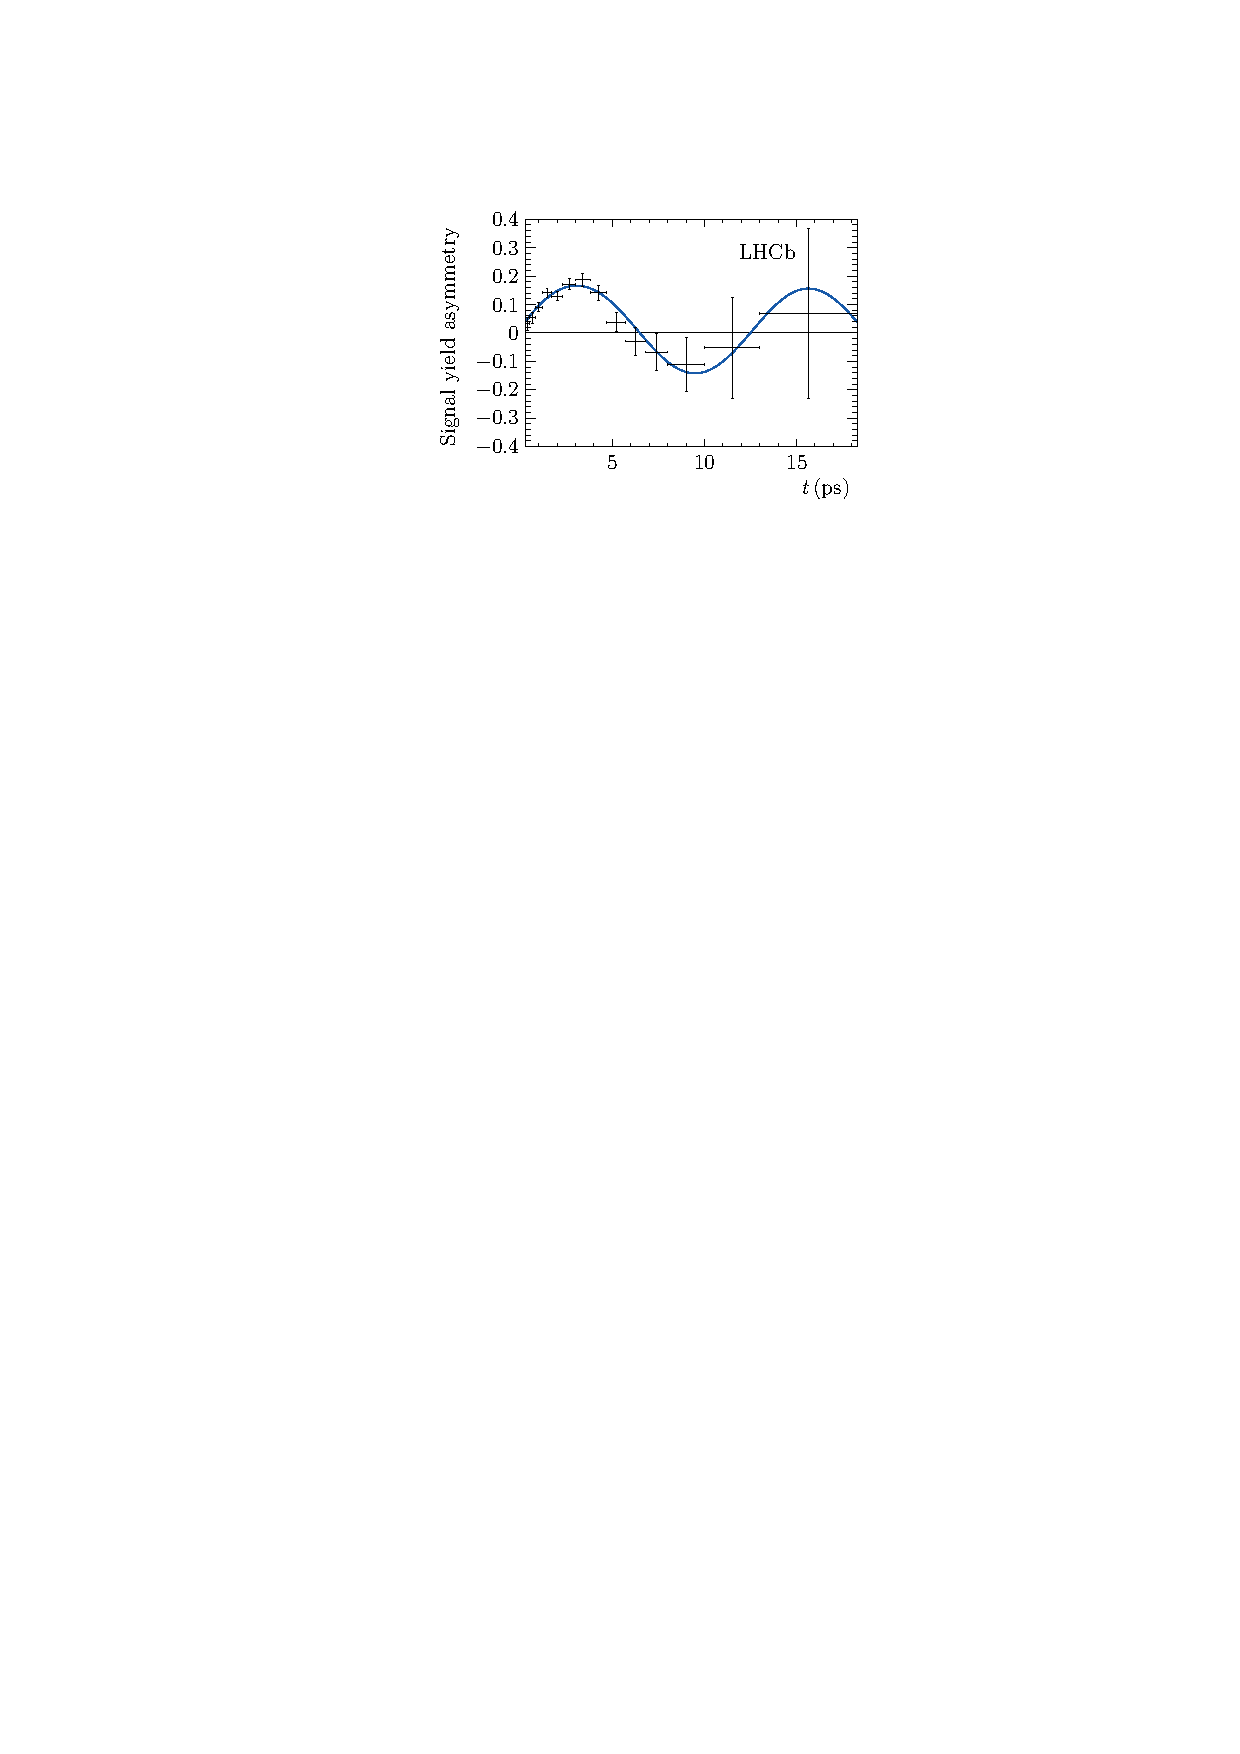
\includegraphics[width=0.266\boxwidth]{CPV_sin2beta.pdf}}
\end{minipage}
\vspace{-0.5em}
}
